%
% File eacl2017_supp.tex
%

\documentclass[11pt]{article}
\usepackage{colacl-onecolumn}
\usepackage{times}
\usepackage{url}
\usepackage{amsmath}
\usepackage{breqn}
\usepackage{latexsym}
\usepackage{pgfplotstable}
\usepackage{algorithm2e}
\usepackage{hhline}
\usepackage{multirow}
\usepackage{multicol}
\usepackage[font=small]{caption}
\usepackage{subcaption}
\usepackage{hyperref}
\usepackage{color}
\usepackage{lipsum,adjustbox}
\usepackage{tikz}
\usepackage{tikz-dependency}
\usepackage{rotating}
\usepackage{float}
\usepackage{xr}
\externaldocument{eacl2016}
\usetikzlibrary{shapes,fit,calc,er,positioning,intersections,decorations.shapes,mindmap,trees}
\tikzset{decorate sep/.style 2 args={decorate,decoration={shape backgrounds,shape=circle,
      shape size=#1,shape sep=#2}}}

\flushbottom \onecolumn

\newcommand{\secref}[1]{Section~\ref{#1}}
\newcommand{\figref}[1]{Figure~\ref{#1}}
\newcommand{\tabref}[1]{Table~\ref{#1}}
\DeclareMathOperator*{\argmin}{argmin}
\DeclareMathOperator*{\argmax}{argmax}
\SetKwRepeat{Do}{do}{while}
\renewcommand\AlCapFnt{\normalfont\small}

\makeatletter
\renewcommand{\paragraph}{
  \@startsection{paragraph}{4}
  {\z@}{.5ex \@plus .5ex \@minus .2ex}{-1em}
  {\normalfont\normalsize\bfseries}
}
\makeatother

\newcommand\BibTeX{B\textsc{ib}\TeX}

\title{Broad-Coverage Semantic Parsing: A Transition-Based Approach \\ Supplementary Material}

\begin{document}
\maketitle



\section{Additional UCCA-annotated examples}

\paragraph{Linkage.}

The following figure demonstrates a linkage relation, omitted from Figure 1a in the paper.

\begin{figure}[h]
  \centering
  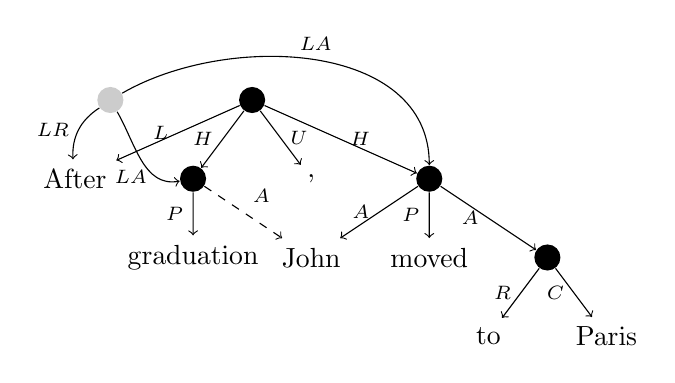
\begin{tikzpicture}[level distance=10mm, ->]
    \node (ROOT) [fill=black, circle] {}
      child {node (After) {After} edge from parent node[left] {\scriptsize $L$}}
      child {node (graduation) [fill=black, circle] {}
      {
        child {node {graduation} edge from parent node[left] {\scriptsize $P$}}
      } edge from parent node[left] {\scriptsize $H$} }
      child {node {,} edge from parent node[right] {\scriptsize $U$}}
      child {node (moved) [fill=black, circle] {}
      {
        child {node (John) {John} edge from parent node[left] {\scriptsize $A$}}
        child {node {moved} edge from parent node[left] {\scriptsize $P$}}
        child {node [fill=black, circle] {}
        {
          child {node {to} edge from parent node[left] {\scriptsize $R$}}
          child {node {Paris} edge from parent node[left] {\scriptsize $C$}}
        } edge from parent node[left] {\scriptsize $A$} }
      } edge from parent node[right] {\scriptsize $H$} }
      ;
    \draw[dashed,->] (graduation) to node [auto] {\scriptsize $A$} (John);
    \node (LKG) at (-1.8,0) [fill=black!20, circle] {};
          \draw[bend right] (LKG) to node [auto, left] {\scriptsize $LR$} (After);
          \draw (LKG) to[out=-60, in=190] node [below] {\scriptsize $LA\quad$} (graduation);
          \draw (LKG) to[out=30, in=90] node [above] {\scriptsize $LA$} (moved);
  \end{tikzpicture}
  \caption{UCCA example with linkage.}
\end{figure}

\paragraph{Longer example.}

The following figure shows the UCCA annotation for the sentence
``A similar technique is almost impossible to apply to other crops, such as cotton, soybeans and rice.''.
The sentence was used by \cite{oepen2015semeval} to compare between the difference schemes.
It includes a single Scene, whose main relation is ``apply'', a secondary relation ``almost impossible'', as well as two complex arguments: ``a similar technique'' and the coordinated argument ``such as cotton, soybeans, and rice.''

\begin{figure}[h]
  \centering
  \scalebox{.6}{
  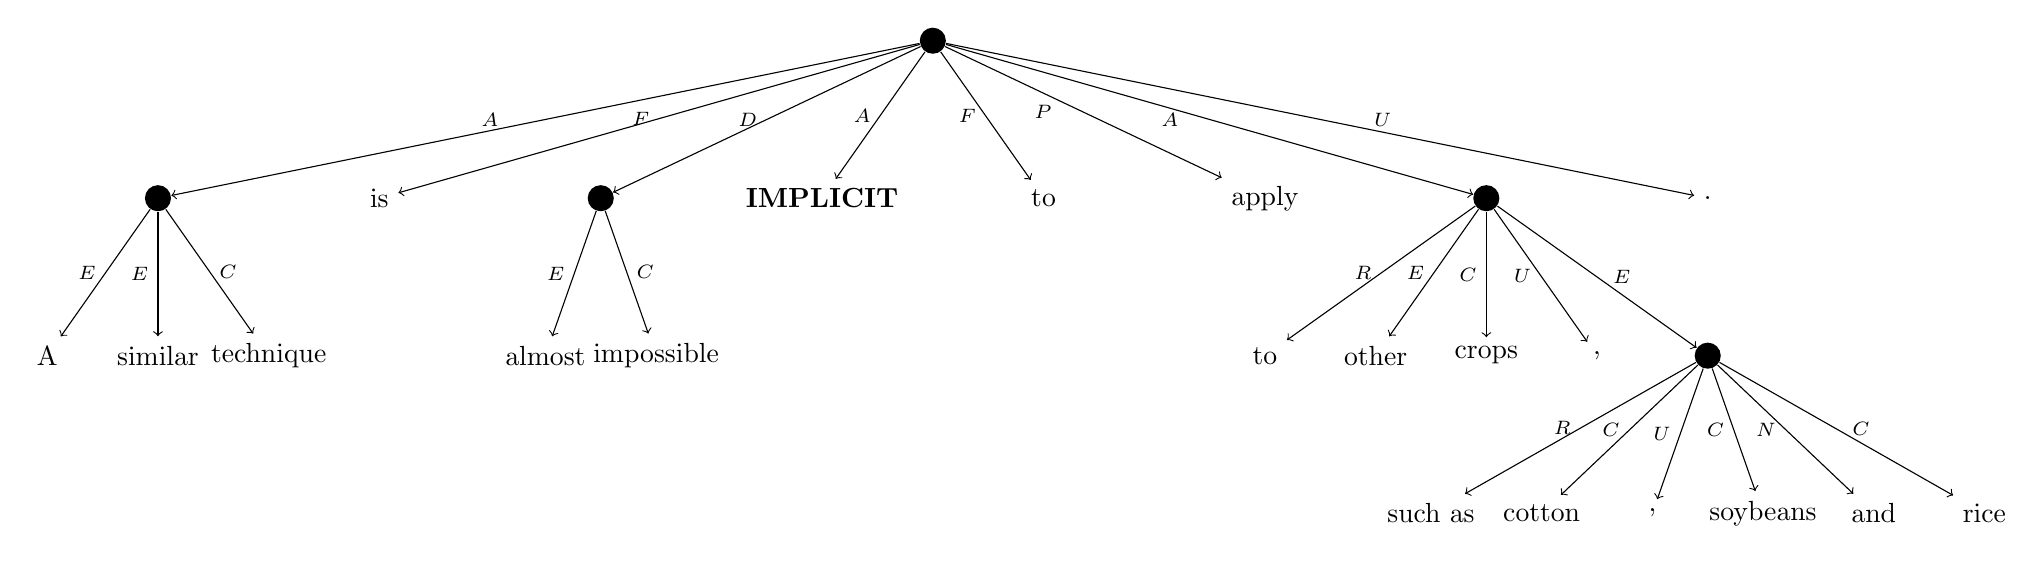
\begin{tikzpicture}[level distance=20mm, ->,
  level 1/.style={sibling distance=8em},
  level 2/.style={sibling distance=4em},
  level 3/.style={sibling distance=4em}]
    \node (ROOT) [fill=black, circle] {}
      child {node [fill=black, circle] {}
      {
        child {node {A} edge from parent node[left] {\scriptsize $E$}}
        child {node {similar} edge from parent node[left] {\scriptsize $E$}}
        child {node {technique} edge from parent node[right] {\scriptsize $C$}}
      } edge from parent node[left] {\scriptsize $A\quad$ \hspace{1mm} } }
      child {node {is} edge from parent node[left] {\scriptsize $F$}}
      child {node [fill=black, circle] {}
      {
        child {node {almost} edge from parent node[left] {\scriptsize $E$}}
        child {node {impossible} edge from parent node[right] {\scriptsize $C$}}
      } edge from parent node[left] {\scriptsize $D$} }
      child {node {\textbf{IMPLICIT}} edge from parent node[left] {\scriptsize $A$}}
      child {node {to} edge from parent node[left] {\scriptsize $F$}}
      child {node {apply} edge from parent node[left] {\scriptsize $P\quad$}}
      child {node [fill=black, circle] {}
      {
        child {node {to} edge from parent node[left] {\scriptsize $R$}}
        child {node {other} edge from parent node[left] {\scriptsize $E$}}
        child {node {crops} edge from parent node[left] {\scriptsize $C$}}
        child {node {,} edge from parent node[left] {\scriptsize $U$}}
        child {node [fill=black, circle] {}
        {
          child {node {such as} edge from parent node[left] {\scriptsize $R$}}
          child {node {cotton} edge from parent node[left] {\scriptsize $C$}}
          child {node {,} edge from parent node[left] {\scriptsize $U$}}
          child {node {soybeans} edge from parent node[left] {\scriptsize $C$}}
          child {node {and} edge from parent node[left] {\scriptsize $N$}}
          child {node {rice} edge from parent node[right] {\scriptsize $\; C$}}
        } edge from parent node[right] {\scriptsize $\; E$ \hspace{1mm} } }
      } edge from parent node[left] {\scriptsize $A\;$ \hspace{1mm} } }
      child {node {.} edge from parent node[right] {\scriptsize $\quad \quad U$}}
      ;
  \end{tikzpicture}
  }
  \caption{Longer UCCA example.}
\end{figure}

\section{Conversion algorithms}

\paragraph{Conversion from constituency to dependency trees.}
Let $T_c=(V_c,E_c,\ell_c)$ be a constituency tree with labels $\ell_c:E_c~\rightarrow~L$.
The conversion from $T_c$ to a dependency tree involves the removal of
all non-terminals from $T_c$ and the addition of edges between terminals.
The nodes of the converted dependency tree are simply the terminals of $T_c$.

We define a linear order over possible edge labels $L$ (\figref{fig:priority}).
For each node $u \in V$, denote by $h(u)$ its child with the highest edge label.
Let $h^*(u)$ be the terminal reached by recursively applying $h(\cdot)$ over $u$.
For each terminal $t$, we define $n(t)$ as the highest
non-terminal such that $t=h^*(n(t))$, i.e.
$n(t)$ is the only node such that $t=h^*(n(t))$ and $t \neq h^*(\mathrm{Parent}_c(n(t)))$.
$t$'s head in the dependency graph is
the terminal $h^*(\mathrm{Parent}_c(n(t)))$.
The complete conversion procedure from constituency to dependency is given in Algorithm~\ref{alg:con2dep}.

Note that this conversion procedure is simpler than the
head percolation procedure used for converting syntactic constituency
trees to dependency trees,
since $h(u)$ (similar to $u$'s head-containing child)
depends only on $\ell_c(h(u),u)$ and not on the sub-tree spanned by $u$,
because edge labels in UCCA directly express the role of the child in the parent unit, and
are thus sufficient for determining which of $u$'s children contains the head node.

\begin{algorithm}[h]
 \KwData{constituency tree ${T_c}=(V_c,E_c,\ell_c)$}
 \KwResult{dependency tree $T_d=(V_d,E_d,\ell_d)$}
 
 \ForEach{$u \in V_c$} {
  $h(u) \leftarrow \argmin_v \mathrm{Priority}(\ell_c(u,v))$\;
 }
 $V_d \leftarrow \mathrm{Terminals}({T_c})$,
 $E_d \leftarrow \emptyset$\;
 \ForEach{$t \in V_d$} {
  $u \leftarrow t$\;
  \While{$u=h(\mathrm{Parent}_c(u))$} {
  	$h^*(u) \leftarrow t$\;
  	$u \leftarrow \mathrm{Parent}_c(u)$\;
  }
  $n(t) \leftarrow h(u)$\;
 }
 \ForEach{$t \in V_d$} {
  $u \leftarrow \mathrm{Parent}_c(n(t))$\;
  $t^\prime \leftarrow h^*(u)$\;
  $E_d \leftarrow E_d \cup \{(t^\prime, t)\}$\;
  $\ell_d (t^\prime, t) \leftarrow \ell_c(u, n(t))\}$\;
 }
 \caption{Constituency to dependency conversion.}
 \label{alg:con2dep}
\end{algorithm}

\paragraph{Conversion from dependency to constituency trees.}
The inverse conversion introduces non-terminal nodes back into the tree.
As the distinction between low- and high-attaching nodes is lost in the constituency to
dependency conversion, we assume that attachments are always
high-attaching.
Let $T_d=(V_d,E_d,\ell_d)$ be a dependency tree.
We begin by creating a root node $r$.
Then, iterating over $V_d$ in topological order,
we add its members as terminals to the constituency tree
and create a pre-terminal parent for each,
with an edge labeled as \textit{Terminal} between them.
The parents of the pre-terminals are determined by the terminal's parent in the dependency
tree: if a dependency node $t$ is a child of the root in $T_d$, then $t$'s pre-terminal will also be a child of the root node. Otherwise, $t$'s pre-terminal is the child of the pre-terminal associated with $t$'s head in $T_d$. We add an intermediate node in between if $t$ has any dependents in $T_d$,
to allow adding their pre-terminals as children.
Edge labels for the intermediate edges are determined by a rule-based function, denoted by $\mathrm{Label}(u)$.
This procedure is given in Algorithm~\ref{alg:dep2con}.

\begin{algorithm}[h]
 \KwData{dependency tree $T_d=(V_d,E_d,\ell_d)$}
 \KwResult{constituency tree $T_c=(V_c,E_c,\ell_c)$}
 \SetKwFunction{Label}{Label}{}{}
 
 $r \leftarrow \mathrm{Node()}$\;
 $V_c \leftarrow \{r\}$,
 $E_c \leftarrow \emptyset$\;
 \ForEach{$t \in \mathrm{TopologicalSort}(V_d)$} {
  $u \leftarrow \mathrm{Node()}$\;
  $V_c \leftarrow V_c \cup \{u, t\}$\;
  $E_c \leftarrow E_c \cup \{(u, t)\}$\;
  $\ell_c(u,t)\leftarrow\mathit{Terminal}$\;
  $t^\prime \leftarrow \mathrm{Parent}_d(t)$\;
  \eIf{$t^\prime = \textsc{Root}$} {
   $E_c \leftarrow E_c \cup \{(r, u)\}$\;
   $\ell_c(r, u) \leftarrow \Label(r)$\;
  } {
   \eIf{$\exists v \in V_d : (t,v) \in E_d$} {
    $u^\prime \leftarrow \mathrm{Node()}$\;
    $E_c \leftarrow E_c \cup \{(u^\prime, u)\}$\;
    $\ell_c(u^\prime, u) \leftarrow \Label(u^\prime)$\;
   } {
    $u' \leftarrow u$\;
   }
   $p \leftarrow \mathrm{Parent}_c(t^\prime)$\;
   $E_c \leftarrow E_c \cup \{(p, u^\prime)\}$\;
   $\ell_c(p, u^\prime) \leftarrow \ell_d(t^\prime, t)$\;
  }
 }
 
  \SetKwProg{func}{Function}{}{}
  
  \func{\Label}{
  \KwData{node $u \in V_d$}
  \KwResult{label $\ell \in L$}

   \uIf{$\mathrm{IsPunctuation}(u)$}{
    \Return \textit{Punctuation}\;
   }
   \uElseIf{$\exists v \in V_d : \ell(u,v) = \textit{ParallelScene}$}{
    \Return \textit{ParallelScene}\;
   }
   \uElseIf{$\exists v \in V_d : \ell(u,v) = \textit{Participant}$}{
    \Return \textit{Process}\;
   }
   \uElse{
    \Return \textit{Center}\;
   }
  }
 \caption{Dependency to constituency conversion.}
 \label{alg:dep2con}
\end{algorithm}

\begin{figure}[h]
\begin{multicols}{2}
\begin{enumerate}
\item $C$ (\textit{Center})
\item $N$ (\textit{Connector})
\item $H$ (\textit{ParallelScene})
\item $P$ \textit{Process})
\item $S$ (\textit{State})
\item $A$ (\textit{Participant})
\item $D$ (\textit{Adverbial})
\item $T$ (\textit{Time})
\item $E$ (\textit{Elaborator})
\item $R$ (\textit{Relator})
\item $F$ (\textit{Function})
\item $L$ (\textit{Linker})
\item $LR$ (\textit{LinkRelation})
\item $LA$ (\textit{LinkArgument})
\item $G$ (\textit{Ground})
\item $\mathit{Terminal}$ (\textit{Terminal})
\item $U$ (\textit{Punctuation})
\end{enumerate}
\end{multicols}
\caption{Priority order of edge labels, used in Algorithm~\ref{alg:con2dep}.}
\label{fig:priority}
\end{figure}


\paragraph{Example.}

Converting the sentence in Figure 1a to a constituency tree consists of simply removing the remote edge, as can be seen in \figref{fig:con_example}.

\begin{figure}[H]
  \centering
  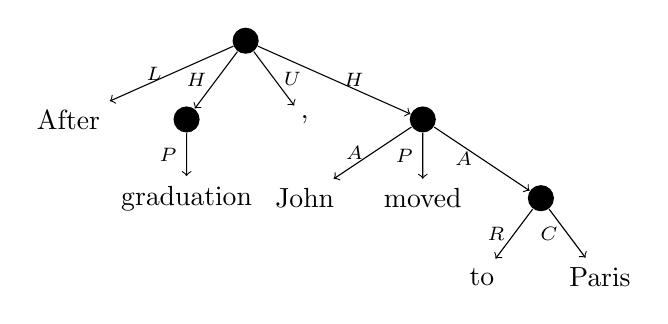
\begin{tikzpicture}[level distance=10mm, ->]
    \node (ROOT) [fill=black, circle] {}
      child {node (After) {After} edge from parent node[left] {\scriptsize $L$}}
      child {node (graduation) [fill=black, circle] {}
      {
        child {node {graduation} edge from parent node[left] {\scriptsize $P$}}
      } edge from parent node[left] {\scriptsize $H$} }
      child {node {,} edge from parent node[right] {\scriptsize $U$}}
      child {node (moved) [fill=black, circle] {}
      {
        child {node (John) {John} edge from parent node[left] {\scriptsize $A$}}
        child {node {moved} edge from parent node[left] {\scriptsize $P$}}
        child {node [fill=black, circle] {}
        {
          child {node {to} edge from parent node[left] {\scriptsize $R$}}
          child {node {Paris} edge from parent node[left] {\scriptsize $C$}}
        } edge from parent node[left] {\scriptsize $A$} }
      } edge from parent node[right] {\scriptsize $H$} }
      ;
  \end{tikzpicture}
  \caption{Example: conversion to constituency tree}
  \label{fig:con_example}
\end{figure}

The corresponding dependency tree is given in \figref{fig:dep_example}.

\begin{figure}[H]
\centering
\begin{dependency}[theme = simple]
\begin{deptext}[column sep=.7em,ampersand replacement=\^]
After \^ graduation \^ , \^ John \^ moved \^ to \^ Paris \\
\end{deptext}
\depedge{2}{1}{L}
\depedge{2}{3}{U}
\depedge{5}{4}{A}
\depedge{2}{5}{H}
\depedge{7}{6}{R}
\depedge{5}{7}{A}
\end{dependency}
  \caption{Example: conversion to dependency tree}
  \label{fig:dep_example}
\end{figure}

\section{Conversion-based out-of-domain results}

The scores in \tabref{tab:ood_converted} were obtained on primary edges when running the conversion-based parsers on the out-of-domain data set (\textit{20K Leagues}). Scores on remote edges are zero, since they are not reconstructed by the conversion.
\begin{table}[H]
  \centering
\begin{tabular}{l|ccc}
& \textbf{LP} & \textbf{LR} & \textbf{LF} \\
\hline
\multicolumn{4}{l}{\rule{0pt}{2ex} \footnotesize Constituency Tree Conversion} \\
\textsc{uparse} & 57 & 59.4 & 58 \\
Upper Bound & 100 & 100 & 100 \\
\hline
\multicolumn{4}{l}{\rule{0pt}{4ex} \footnotesize Dependency Tree Conversion} \\
Malt$_{\textrm{arc-standard}}$ & 62.3 & 55.9 & 58.7 \\
Malt$_{\textrm{arc-eager}}$ & 62.8 & 56.3 & 59.2 \\
LSTM & {\bf 70.1} & {\bf 63.3} & {\bf 66.1} \\
Upper Bound & 93.5 & 82.5 & 87.6 \\
\end{tabular}
\caption{Results for conversion-based parsing when tested on out-of-domain data (\textit{20K Leagues})}
\label{tab:ood_converted}
\end{table}

\section{Feature ablation experimental results}

The following results, in percents,
were obtained on the development set in the feature ablation experiment (Section 7 in the paper).
The first row corresponds to \textsc{bsp} as in the main experiment.
In each of the other rows, one feature set is excluded.
Columns are the same as in Table 2 in the paper.
See Section 5 and Figure 3 in the paper for the feature set definitions.
  
\begin{table}[H]
\centering
\begin{tabular}{l|ccc|ccc}
& \multicolumn{3}{c|}{Primary} & \multicolumn{3}{c}{Remote} \\
& \textbf{LP} & \textbf{LR} & \textbf{LF} & \textbf{LP} & \textbf{LR} & \textbf{LF} \\
\hline
\textsc{bsp} & 62.6	& 55.7 & 58.9 & 20 & 12.9 & 15.7 \\
\textsc{bsp}$-$\textbf{unigrams} & 62.5 & 52.6 & 57.1 & 18.9 & 10.1 & 13.2 \\
\textsc{bsp}$-$\textbf{bigrams} & 59.8 & 50.0 & 54.4 & 18.2 & 12.2 & 14.6 \\
\textsc{bsp}$-$\textbf{trigrams} & 63.7 & 55.0 & 59.0 & 20.7 & 12.0 & 15.2 \\
\textsc{bsp}$-$\textbf{separator} & 62.9 & 53.5 & 57.8 & 17.8 & 11.7 & 14.1 \\
\textsc{bsp}$-$\textbf{extended} & 62.9 & 52.8 & 57.4 & 17.4 & 11.5 & 13.9 \\
\textsc{bsp}$-$\textbf{disco} & 63.6 & 53.6 & 58.2 & 19.7 & 11.5 & 14.5 \\
\textsc{bsp}$-$\textbf{counts} & 63.3 & 52.8 & 57.6 & 14.6 & 10.6 & 12.3 \\
\textsc{bsp}$-$\textbf{edges} & 63.5 & 54.9 & 58.9 & 23.6 & 14.5 & 17.9 \\
\textsc{bsp}$-$\textbf{history} & 63.1 & 53.2 & 57.8 & 23.7 & 14.5 & 18.0 \\
\textsc{bsp}$-$\textbf{remote} & 63.5 & 53.2 & 57.9 & 17.2 & 10.6 & 13.1 \\
\textsc{bsp}$-$\textbf{ratio} & 63.7 & 48.3 & 55.0 & 25.4 & 13.6 & 17.7
\end{tabular}
\caption{Results for feature ablation experiments.}
\label{tab:ablation}
\end{table}


\bibliography{references}
\bibliographystyle{eacl2017}

\end{document}
